\documentclass[11pt]{amsart}
\usepackage[margin=1.15in]{geometry}
\usepackage{amssymb,amsmath,mathtools}
\usepackage{graphicx}
\usepackage{booktabs}
\usepackage{enumitem}
\usepackage[hidelinks]{hyperref}
\usepackage{xcolor}

\newtheorem{theorem}{Theorem}
\renewcommand{\thetheorem}{\Alph{theorem}}
\newtheorem{thm}{Theorem}[section]
\newtheorem{lemma}[thm]{Lemma}
\newtheorem{proposition}[thm]{Proposition}
\newtheorem{corollary}[thm]{Corollary}
\theoremstyle{definition}
\newtheorem{definition}[thm]{Definition}
\newtheorem{remark}[thm]{Remark}
\newtheorem{example}[thm]{Example}
\newtheorem{question}[thm]{Question}

\newcommand{\R}{\mathbb{R}}
\newcommand{\Q}{\mathbb{Q}}
\newcommand{\Z}{\mathbb{Z}}
\newcommand{\msum}{\oplus}
\DeclareMathOperator{\conv}{conv}
\DeclareMathOperator{\vol}{vol}
\DeclareMathOperator{\SO}{SO}

\title[Minkowski sums of simplices that tile space]{Minkowski sums of triangles and segments that tile space, and equilateral space-fillers}
\author{Vladimir Muravev}
\date{October 9, 2026}

\begin{document}
\begin{abstract}
We study convex polyhedra $P = \Delta_1 \msum \dots \msum \Delta_k \subset \R^3$ that are Minkowski sums of
segments and triangles in general position. We prove that if the total dimension $\sum \dim \Delta_i$ is
$4$, then $P$ tiles $\R^3$ by translates of $P$ and of its point reflection; the proof is an exact
computer-assisted verification of Poincar\'e's polyhedron theorem on every chamber of the configuration space,
followed by a limit argument that extends the result to every position in which $P$ is three-dimensional. Together with
the classical cases this shows that every such sum with $\sum\dim\Delta_i\le 4$ tiles space. Conversely, if the
summands are unit segments and unit equilateral triangles and $\sum \dim \Delta_i \geq 5$, we prove that in every
chamber the members that tile $\R^3$ by congruent copies (with arbitrary isometries) form a set of measure zero.
The key ingredient is an independence lemma for dihedral angles, proved by a monodromy argument, which reduces
every identity among the dihedral angles of $P$ to a circulation in a graph attached to each zone.

As a consequence we obtain two new families of equilateral convex space-fillers, with $9$ faces
(four triangles and five rhombi) and $10$ faces (two triangles and eight rhombi). We also report on a
classification attempt for equilateral convex polyhedra with at most $8$ faces that tile space, which is
rigorous for $170$ of the $301$ combinatorial types and numerical for the rest.
\end{abstract}
\maketitle

\section{Introduction}

Which convex polygons with all sides equal tile the plane? The question goes back to the classification of
convex pentagonal tiles. Hirschhorn and Hunt~\cite{HH85} determined the equilateral convex pentagons that tile,
Rao's computer search~\cite{Rao17} completed the list of convex pentagonal tiles, and Klaassen~\cite{Kla25}
recently gave a short self-contained answer: an equilateral convex polygon tiles the plane if and only if it is
a triangle, a quadrilateral, a pentagon with two angles summing to $\pi$ or similar to a particular pentagon $P_7$,
or a hexagon with three distinct angles summing to $2\pi$, two of which share an edge.

The three-dimensional analogue asks for the \emph{equilateral} convex polyhedra (all edges of the same length)
that tile $\R^3$ by congruent copies. We are not aware of a classification even in small cases. Classical
examples are the cube, the rhombic parallelepipeds, the triangular and hexagonal prisms, the rhombic
dodecahedron, the truncated octahedron and the gyrobifastigium (Johnson solid $J_{26}$~\cite{Joh66}). This paper grew out of an
attempt to classify the equilateral space-fillers with at most $8$ faces. That search showed that every
positive-dimensional family of such tiles we found is a Minkowski sum of unit segments and unit triangles. This
led us to study such sums in general.

\subsection*{Setting}
Let $\Delta_1, \dots, \Delta_k \subset \R^3$ be segments and triangles, and $P = \Delta_1 \msum \dots \msum
\Delta_k$. The \emph{total dimension} of the sum is $\sum_i \dim \Delta_i$. The sum is in \emph{general position} if
every $3\times 3$ determinant formed by edge vectors of three distinct summand edges, not all from the same
triangle, is non-zero. For fixed types of summands, the general-position configurations form an open set; its
connected components are the \emph{chambers}. On a chamber the combinatorial type of $P$ is constant.

\begin{theorem}\label{thm:A}
Let $P$ be the Minkowski sum of two triangles, or of a parallelogram and a triangle, and assume that $P$ is
three-dimensional. Then $P$ tiles $\R^3$ by translates of $P$ and of its point reflection $-P$. Explicitly, the
images of $P$ under a group generated by a lattice $L$ and one point reflection $x\mapsto w-x$, with $L$ and $w$ given in
Table~\ref{tab:lattices}, form a tiling. For summands in general position the tiling is face-to-face.
\end{theorem}

Combined with the classical cases (parallelepipeds, triangular prisms, and McMullen's theorem that zonotopes
with four generators in general position are parallelohedra~\cite{McM75}), Theorem~\ref{thm:A} shows:

\begin{corollary}\label{cor:le4}
Every Minkowski sum of segments and triangles in general position in $\R^3$ with total dimension $3$ or $4$ tiles
space by translations and point reflections.
\end{corollary}

\begin{theorem}\label{thm:B}
Fix a type of Minkowski sum of unit segments and unit equilateral triangles in $\R^3$ with total dimension at
least $5$, and let $\mathcal{C}$ be a chamber of its configuration space (the rotations of the summands). Then
the set of $P\in\mathcal{C}$ that tile $\R^3$ by congruent copies, with arbitrary isometries and not necessarily
face-to-face, has measure zero in $\mathcal{C}$.
\end{theorem}

The dimension bound is sharp in the sense of Corollary~\ref{cor:le4}. The general-position hypothesis is
essential: in special positions, sums of total dimension $5$ can tile (Example~\ref{ex:elongated}), and
Theorem~\ref{thm:B} gives no information about the exceptional set of measure zero.
Theorems~\ref{thm:A} and~\ref{thm:B} parallel McMullen's criterion for zonotopes, where four generic generators
give a parallelohedron and five do not. In our setting the threshold is the total dimension $d+1 = 4$, and
Theorem~\ref{thm:B} excludes tilings by arbitrary isometries, not only translations.

\subsection*{Equilateral consequences}
Taking unit summands, Theorem~\ref{thm:A} produces equilateral convex space-fillers
(Figure~\ref{fig:bodies}).
\begin{itemize}[leftmargin=2em]
\item Two triangles in the $8$-face chamber give the \emph{generalized gyrobifastigium}: two oblique triangular
prisms glued along a rhombus. It is a $3$-parameter family containing $J_{26}$.
\item Two triangles in the $9$-face chamber give a $3$-parameter family with four triangles and five rhombi.
\item A rhombus and a triangle give a $4$-parameter family with $10$ faces (two triangles and eight rhombi).
\end{itemize}
To our knowledge the $9$- and $10$-face families have not appeared in the literature as space-fillers.

\begin{figure}[t]
\centering
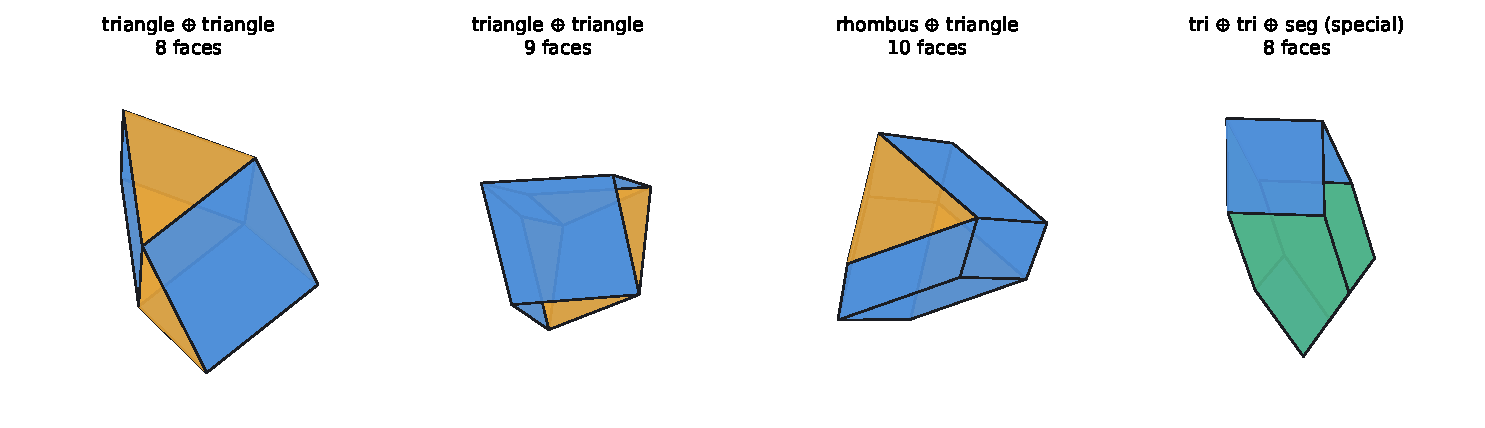
\includegraphics[width=\textwidth]{fig_bodies.pdf}
\caption{Equilateral space-fillers that are Minkowski sums of unit triangles and segments. From left to right:
triangle $\msum$ triangle in the $8$-face chamber (generalized gyrobifastigium) and in the $9$-face chamber;
rhombus $\msum$ triangle ($10$ faces); a special position of triangle $\msum$ triangle $\msum$ segment
(generalized elongated gyrobifastigium, Example~\ref{ex:elongated}). Triangles are orange, rhombi blue, pentagons
green.}\label{fig:bodies}
\end{figure}

\subsection*{Methods and rigour}
The proof of Theorem~\ref{thm:A} is computer-assisted but exact: every check is an identity of
polynomials with rational coefficients or a sign condition decided by finitely many exact evaluations. The proof
of Theorem~\ref{thm:B} is conceptual; the computations reported alongside it (exact rank checks,
an exhaustive check of arrangements, interval certificates) serve as independent confirmation. All code is publicly available~\cite{code}.

\subsection*{Organisation}
Section~\ref{sec:prelim} collects the dihedral-angle and Dehn-invariant obstructions and the zone structure of
Minkowski sums. Section~\ref{sec:A} proves Theorem~\ref{thm:A}, and Section~\ref{sec:B} proves Theorem~\ref{thm:B}.
Section~\ref{sec:class} reports the status of the classification of equilateral space-fillers with at most $8$
faces. Section~\ref{sec:open} lists open problems.

\section{Preliminaries}\label{sec:prelim}

\subsection{Two obstructions}
Let $P$ be a convex polytope with dihedral angles $\theta_e\in(0,\pi)$, $e$ an edge.

\begin{lemma}[dihedral filter]\label{lem:filter}
If $P$ tiles $\R^3$ by congruent copies, then for every edge $e$ of $P$ there are non-negative integers $k_f$ ($f$
an edge of $P$) with $k_e\ge1$ and
\[ \sum_f k_f\theta_f \in\{\pi, 2\pi\}. \]
\end{lemma}
\begin{proof}
Take a point $x$ in the relative interior of $e$, generic in the tiling. The tiles containing $x$ fill a small
ball around $x$. Each of them contains $x$ either in the relative interior of an edge, contributing its dihedral
angle there, or in the relative interior of a face, contributing $\pi$. At most one tile can contain $x$ in a
face interior, since two such tiles would leave no room for the tile containing $e$. Since congruent copies, including
mirror images, have the same multiset of dihedral angles, the angles of the first kind sum to $2\pi$ or $\pi$.
\end{proof}

\begin{lemma}[Dehn invariant]\label{lem:dehn}
If $P$ is equilateral with edge length $1$ and tiles $\R^3$ by congruent copies, then $\sum_e \theta_e \in \Q\pi$.
\end{lemma}
\begin{proof}
A polytope that tiles space by congruent copies has vanishing Dehn invariant (Debrunner~\cite{Deb80};
Lagarias--Moews~\cite{LM95}). For an equilateral polytope $D(P)=\sum_e 1\otimes\theta_e = 1\otimes\sum_e\theta_e$ in
$\R\otimes_\Z \R/\pi\Q$, which vanishes if and only if $\sum_e\theta_e\in\Q\pi$.
\end{proof}

\subsection{Zones of Minkowski sums}\label{sec:zones}
Let $P = \Delta_1\msum\dots\msum\Delta_k$ be in general position. Every face of $P$ is either a parallelogram
$a\msum b$, where $a,b$ are edges of two different summands, or a translate of a triangle summand. Every edge of $P$
is a translate of an edge of some summand. For an edge direction $d$ of a summand, the \emph{zone} of $d$ is the set of
faces of $P$ that contain an edge parallel to $d$. The zone of a segment is a closed belt. The zone of a triangle edge
is a chain that starts and ends at the two copies of the triangle that contain this edge.

Fix $d$ and project along $d$. Every face of the zone of $d$ projects to a segment. For a parallelogram $d\msum x$ the
segment is parallel to the projection of $x$. For a copy of the triangle containing $d$ the segment is parallel to the
projection of its plane. We call $x$, respectively the triangle plane, the \emph{line seen from $d$} by that face. If
an edge parallel to $d$ separates faces seeing $a$ and $b$, its dihedral angle is
\begin{equation}\label{eq:angle}
\theta = \pi - \angle_d(a,b),
\end{equation}
where $\angle_d(a,b)\in(0,\pi)$ is the oriented angle from the projection of $a$ to that of $b$ in the plane
$d^\perp$, measured in the direction of travel along the zone. Fixing a reference line $x_0$ seen from $d$, we write
$A_d(x) = \angle_d(x_0,x)$ for the \emph{argument functions}. Every dihedral angle of $P$ is a difference of two
argument functions plus a multiple of $\pi$.

\begin{definition}
The \emph{formula graph} $G_d$ of the zone of $d$ is the directed graph whose vertices are the lines seen from $d$
and whose arcs are the distinct ordered pairs $(a,b)$ of lines seen by consecutive faces of the zone, in the
direction of travel. Each arc $\alpha=(a,b)$ carries the angle $\varphi_\alpha = \angle_d(a,b)$, and all edges of $P$
on this arc have dihedral angle $\pi-\varphi_\alpha$. The \emph{value} of a directed cycle $\gamma$ in $G_d$ is
$\sum_{\alpha\in\gamma}(\pi-\varphi_\alpha)$.
\end{definition}

For a directed cycle the angles $\varphi_\alpha$ sum to a multiple of $\pi$, because the lines return to the starting
line. Each term $\pi-\varphi_\alpha$ is positive, so \textbf{every directed cycle has value at least $\pi$}, and its
value is a multiple of $\pi$. Following the whole zone gives $\sum \varphi = \pi$ for a triangle edge, where the
travel turns the plane of the triangle by a half-turn, and $\sum\varphi = 2\pi$ for a segment belt.

\section{Proof of Theorem~\ref{thm:A}}\label{sec:A}

\subsection{Affine normalisation}
If $\Gamma$ is generated by a lattice and a point reflection and $\Gamma P$ is a tiling, then for every affine
bijection $g$ the group $g\Gamma g^{-1}$ is again of this form and tiles by $gP$. Hence we may normalise
\[
T_1=\{0,e_1,e_2\},\quad T_2=\{0,e_3,v\}\qquad\text{or}\qquad
\Pi=\{0,e_1,e_1+e_2,e_2\},\quad T=\{0,e_3,v\},
\]
convex hulls understood, with $v=(a,b,c)$. Every pair of summands in general position is affinely equivalent to
one of these. General position is the non-vanishing of the linear forms
\[
a,\ b,\ a+b,\ c,\ c-1 \quad(\text{two triangles}),\qquad a,\ b,\ c,\ c-1 \quad (\text{parallelogram and triangle}).
\]
The complements of their zero sets consist of $18$, respectively $12$, open regions. These are the chambers. Each is the product of a sector in the $(a,b)$-plane with an
interval or half-line in $c$.

\subsection{Linear certificates}
Every vertex of $P$ is a sum of summand vertices and is affine-linear in $v$. Every determinant that defines a face
plane, or the side of a vertex with respect to a plane, contains the vector $v$ in at most one column. Hence all
supporting and separating forms that occur are affine-linear in $(a,b,c)$. An affine-linear function is positive on a
chamber if and only if it is non-negative at the vertices of the chamber's closure and on its recession rays, and not
identically zero. This is a finite exact test.

\subsection{Poincar\'e's theorem}
We use the Euclidean case of Poincar\'e's polyhedron theorem~\cite{EP94}: let $P$ be a compact convex polytope with
a pairing $F\mapsto F'$ of its faces and isometries $\gamma_F$ with $\gamma_F(F')=F$ and $\gamma_{F'}=\gamma_F^{-1}$,
such that $\gamma_F P$ and $P$ lie on opposite sides of $F$. Suppose moreover that every edge cycle closes up with
trivial holonomy and angle sum $2\pi$. Then $P$ is a fundamental domain of the group generated by the $\gamma_F$, and its
images tile space face-to-face. Our pairings are translations and point reflections $x\mapsto\pm x+t$, which are
Euclidean isometries in the normalised coordinates, so the theorem applies directly.

For each chamber, our prover \texttt{prove\_tiling.py}~\cite{code} computes the combinatorics of $P$ at a sample point,
proposes the group of Table~\ref{tab:lattices}, and checks the following.
\begin{enumerate}[label=(\roman*),leftmargin=2.5em]
\item Every face $F$ lies in a supporting plane: the defining form vanishes identically on $F$ and is negative on
all other vertices, on the whole chamber.
\item For every face $F$ there is a face $G$ and $\gamma_F\in\Gamma$ with $\gamma_F(G)=F$, as a symbolic identity in
$(a,b,c)$, and $\gamma_F P$ lies strictly on the other side of $F$, by linear certificates.
\item[(ii$'$)] The pairing of $G$ is $\gamma_F^{-1}$.
\item[(iii)] Around every edge the cycle of pairings returns with trivial holonomy, as a symbolic identity. The
dihedral angles along the cycle are continuous on the chamber and sum to a multiple of $2\pi$. They sum to $2\pi$ at the
sample point, hence on the whole chamber.
\end{enumerate}
All $18$ chambers for two triangles and all $12$ chambers for the parallelogram and the triangle pass, in about $50$
seconds in total. One formula of Table~\ref{tab:lattices} serves every chamber of the same face count.

\begin{table}[t]
\centering
\renewcommand{\arraystretch}{1.25}
\begin{tabular}{@{}lll@{}}
\toprule
Body & Lattice $L$ & Point reflection $x\mapsto w-x$ \\
\midrule
$T_1\msum T_2$, $8$ faces & $\langle v_1,\ u_1,\ u_2-v_2\rangle$ & $w = 2(o_1+o_2)+v_1+u_1+u_2$ \\
$T_1\msum T_2$, $9$ faces & $\langle u_1+v_1,\ u_1+v_2,\ u_2-u_1\rangle$ & $w = 2(o_1+o_2)$ \\
$\Pi\msum T$, $10$ faces & $\langle r_1+r_2+t_1,\ r_1+r_2+t_2,\ r_1-r_2+t_1-t_2\rangle$ & $w=2(o+o_T)+r_1+t_1$\\
\bottomrule
\end{tabular}
\medskip
\caption{Tilings of Theorem~\ref{thm:A}. Here $T_1=o_1+\conv\{0,u_1,u_2\}$, $T_2=o_2+\conv\{0,v_1,v_2\}$,
$\Pi = o+\conv\{0,r_1,r_2,r_1+r_2\}$ and $T=o_T+\conv\{0,t_1,t_2\}$, for a suitable labelling of the vertices. In each
case $|\det L| = 2\vol P$.}\label{tab:lattices}
\end{table}

\subsection{Special positions}
On the walls between chambers the tilings stop being face-to-face. For example, a triangle and an adjacent rhombus
become coplanar and merge into a pentagon, and a neighbouring tile meets only the rhombus part. Poincar\'e's
theorem then does not apply verbatim. A limit argument handles this.

\begin{lemma}[limit lemma]\label{lem:limit}
Let $P_t\to P_0$ in the Hausdorff metric as $t\to 0^+$, with $P_0$ three-dimensional. Let $\Gamma_t$ be
generated by a lattice $L_t$ and the point reflection $x\mapsto w_t-x$, where $L_t\to L_0$ and $w_t\to w_0$, and
identify the elements of all $\Gamma_t$ by their integer coordinates. If $\Gamma_t P_t$ is a tiling for every $t>0$,
then $\Gamma_0P_0$ is a tiling.
\end{lemma}
\begin{proof}
For $t>0$ the tiling property gives $|\det L_t| = 2\vol P_t$. In the limit $|\det L_0| = 2\vol P_0>0$, so $L_0$ is a
lattice.

\emph{Covering.} Let $x\in\R^3$. For small $t$ choose $\gamma_t$ with $x\in\gamma_tP_t$. Since the $P_t$ are uniformly
bounded, the integer data of $\gamma_t$ are bounded. Along a sequence $t_n\to0$ they are constant, equal to some
$\gamma$. Then $x\in\gamma_0P_0$, because the tiles are closed and depend continuously on $t$.

\emph{Disjoint interiors.} Suppose $\gamma\ne\gamma'$ and $\gamma_0P_0$, $\gamma'_0P_0$ share an interior point.
Then they contain a common ball $B$. For small $t$ the tiles $\gamma_tP_t$ and $\gamma'_tP_t$ both contain a smaller
concentric ball, which contradicts the tiling property for $t>0$.
\end{proof}

Since one formula works on the whole of each chamber, the lemma extends it to the closure of the chamber,
minus the locus where $P$ degenerates. In the normalisation above, $P$ degenerates only if $a=b=0$. This proves
Theorem~\ref{thm:A}. In particular, the classical gyrobifastigium and the special positions found in our enumeration
(Section~\ref{sec:class}) tile by the formulas of Table~\ref{tab:lattices}.
Figure~\ref{fig:tiling} shows part of a tiling in the $9$-face chamber.

\begin{figure}[t]
\centering
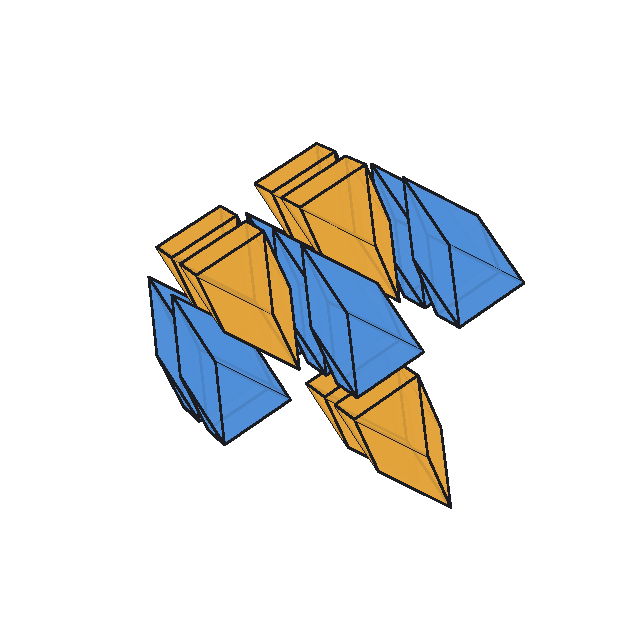
\includegraphics[width=0.55\textwidth]{fig_tiling.pdf}
\caption{Part of the tiling by an equilateral $9$-face triangle $\msum$ triangle, exploded for visibility. Blue
tiles are translates of $P$, and orange tiles are point reflections.}\label{fig:tiling}
\end{figure}

\section{Proof of Theorem~\ref{thm:B}}\label{sec:B}

Throughout this section the summands are a unit segment $s_0$ or a unit equilateral triangle $\Delta_0$, each rotated
by an element of $\SO(3)$. The first summand is fixed, so the configuration space is $\SO(3)^{k-1}$. The general
position locus is open, and its complement is a proper real-algebraic subset.

\subsection{Independence of the argument functions}
Let $d$ run over the edge directions of all summands, and let $x$ run over the lines seen from $d$: the edges of
the other summands and, if $d$ is a triangle edge, the plane of its own triangle. The argument functions
$A_d(x)$ are multivalued real-analytic functions on the configuration space minus the loci $\{x=\pm d\}$.

\begin{lemma}[independence lemma]\label{lem:indep}
Let $\mathcal{C}$ be a chamber. Suppose that real numbers $c_{d,x}$ satisfy
$\sum_{d,x}c_{d,x}A_d(x)\equiv\mathrm{const}$ on $\mathcal{C}$. Then all $c_{d,x}$ vanish.
\end{lemma}

\begin{proof}
It is convenient to replace $A_d(x)$ by the azimuth $\mathrm{az}_d(x)$ of $x$ about $d$ in some frame of $d^\perp$.
Then $A_d(x)=\mathrm{az}_d(x)-\mathrm{az}_d(x_0)$, and the relation becomes $\sum c'_{d,x}\,\mathrm{az}_d(x)\equiv
\mathrm{const}$ with $\sum_xc'_{d,x}=0$ for every $d$. This zero-sum condition makes the relation independent of the
choice of frames.

\emph{Step 1: continuation.} The differential of the left-hand side is a single-valued real-analytic $1$-form on the
complement $U$ of the loci $\{x=\pm d\}$, and it vanishes on the open set $\mathcal C$. Each locus has codimension
$2$ in $\SO(3)^{k-1}$, so $U$ is connected, and the form vanishes on all of $U$.

\emph{Step 2: monodromy.} Along any loop in $U$, the left-hand side returns to its initial value. Each term changes by
$2\pi$ times its coefficient times its winding number. Hence $\sum c'\cdot\mathrm{winding}=0$ for every loop.

\emph{Step 3: test loops.} Let $x$ be an edge direction of summand $j$ and $d$ an edge direction of another summand.
Rotate summand $j$ so that $x$ runs once around a small positive circle about $d$, with the other directions of
summand $j$ remaining generic. Then:
\begin{itemize}[leftmargin=3em]
\item[(W1)] the azimuth of the moving direction $x$ about the fixed pole $d$ winds $+1$;
\item[(W2)] the azimuth of the fixed line $d$ about the moving pole $x$ winds $+1$ as well;
\item no other term winds. Frame rotations at $x$ affect all terms $\mathrm{az}_x(\cdot)$ equally and cancel by the
zero-sum condition.
\end{itemize}
Repeating the loop around $-d$ gives windings $-1$ for (W1) and $+1$ for (W2). Indeed, seen from the pole $d$, a
positive loop around $-d$ is negatively oriented; whereas from the moving pole $x$ near $-d$, the direction $d$ is the
negative of $-d$, which shifts its azimuth by $\pi$ but does not change its winding. We obtain
\[
c'_{d,x}+c'_{x,d}=0,\qquad -c'_{d,x}+c'_{x,d}=0,
\]
so $c'_{d,x}=c'_{x,d}=0$. Thus every coefficient pairing directions of different summands vanishes. For a triangle
edge $d$, the only remaining line seen from $d$ is its own triangle plane, whose coefficient vanishes by the
zero-sum condition.
\end{proof}

The windings (W1) and (W2) were also confirmed numerically. As an independent check, we verified the lemma
by exact rank computations over $\Q$ for nine types (see Remark~\ref{rem:rank}).

\begin{remark}\label{rem:rank}
With rational Cayley rotations and the triangle $\conv\{e_1,e_2,e_3\}$, every gradient of an argument function
is a rational vector up to a constant factor. Stacking gradients at a few rational points, \texttt{independence.py}
finds full rank for tri$+$tri ($18$ functions), tri$+$seg$^2$ ($12$), tri$^2+$seg ($29$), tri$+$seg$^3$ ($21$),
seg$^5$ ($15$), tri$^3$ ($54$), tri$^2+$seg$^2$ ($42$), tri$+$seg$^4$ ($32$) and seg$^6$ ($24$).
\end{remark}

\begin{corollary}\label{cor:circ}
Every identity $\sum_e k_e\theta_e\equiv\mathrm{const}$ on a chamber, with integer $k_e$, is a circulation in the formula
graphs: for each zone $d$, the weights $K_\alpha=\sum_{e\text{ on }\alpha}k_e$ on the arcs of $G_d$ satisfy flow
conservation at every vertex. Consequently an edge $e$ satisfies the dihedral filter identically on a chamber,
that is, some relation of Lemma~\ref{lem:filter} holds as an identity, if and only if the arc of $e$ lies on a directed
cycle of $G_d$ of value at most $2\pi$.
\end{corollary}
\begin{proof}
By~\eqref{eq:angle}, $\sum_e k_e\theta_e = \mathrm{const}-\sum_d\sum_\alpha K_\alpha(A_d(b_\alpha)-A_d(a_\alpha))$, where
$\alpha=(a_\alpha,b_\alpha)$. By Lemma~\ref{lem:indep} the coefficient of each $A_d(x)$ vanishes. This is exactly flow
conservation at $x$. A non-negative integer circulation decomposes into directed cycles. If its value is
$\pi$ or $2\pi$, then every cycle in the decomposition has value at most $2\pi$, since each cycle has value at least
$\pi$. Conversely, a directed cycle of value $\pi$ or $2\pi$ through the arc of $e$ is itself such an identity.
\end{proof}

We call an edge a \emph{witness} on a chamber if its arc lies on no directed cycle of value at most $2\pi$.

\subsection{Witness edges}
On the Gauss sphere, the normal fan of a segment summand is a great circle, and the normal fan of a triangle summand is a
\emph{tripod}: three great semicircles from the normal $n$ to $-n$, perpendicular to its edges. The faces of the zone of a
triangle edge $e$ correspond to the intersections of the semicircle of $e$ with the fans of the other summands.

\begin{lemma}[witness lemma]\label{lem:witness}
If $\sum\dim\Delta_i\ge5$, then every chamber has a witness edge.
\end{lemma}
\begin{proof}
There are three cases.

\emph{(A) At least two triangles $T_i,T_j$ and at least three summands.} The sum $T_i\msum T_j$ has $8$ or $9$
faces (Section~\ref{sec:A}), so the tripods of $T_i$ and $T_j$ cross $4$ or $5$ times. Hence some semicircle
of an edge $e$ of $T_i$ is crossed twice by the tripod of $T_j$. A third summand crosses the semicircle of $e$ at least
once. A great circle of a segment meets the semicircle exactly once. The three lunes cut out by a tripod have angles
less than $\pi$, so no closed lune contains a pair of antipodal points other than its own vertices; hence the semicircle,
whose endpoints are antipodal, cannot avoid the tripod. Two semicircles on distinct great circles meet at most once. The zone of $e$ therefore has at least $4$
arcs. These see pairwise distinct lines and return to the own plane of $T_i$, so $G_e$ is a single directed cycle with
total $\sum\varphi=\pi$. Its value is $(m-1)\pi\ge3\pi$, where $m\ge4$ is the number of arcs, and every edge of the
zone is a witness.

\emph{(B) Exactly one triangle $T$ and $S\ge3$ segments.} The great circle of each segment meets the semicircle of
an edge $e$ of $T$ exactly once, and in general position these intersections are distinct. The zone of $e$ is
the simple cycle (own plane)$\,\to s_1\to\dots\to s_S\to\,$(own plane), with $S+1$ arcs and value $S\pi\ge3\pi$. We
also verified exhaustively all abstract cyclic arrangements for $S\in\{3,4,5\}$ (\texttt{case\_b.py}).

\emph{(C) Only segments, $n\ge5$ of them.} The belt of a segment $s_1$ sees each other segment twice, at antipodal
positions. Its formula graph is a single directed cycle on $n-1$ vertices with $\sum\varphi=\pi$ over one cycle,
so its value is $(n-1)\pi-\pi=(n-2)\pi\ge3\pi$.
\end{proof}

For total dimension at most $4$ the same criterion covers every edge (for example, one triangle and $S\le2$
segments gives value $S\pi\le2\pi$). This agrees with Theorem~\ref{thm:A}. A direct high-precision search for angle
identities agreed with the prediction of Corollary~\ref{cor:circ} on $56$ out of $56$ random members of seven types
(\texttt{zone\_graphs.py}).

\subsection{Measure zero}
Let $e$ be a witness edge on the chamber $\mathcal{C}$. For each integer vector $k\ge0$ with $k_e\ge1$ and each
target $\tau\in\{\pi,2\pi\}$, the function $\sum_fk_f\theta_f-\tau$ is real-analytic on the connected open set
$\mathcal C$. It is not identically zero, by Corollary~\ref{cor:circ}. Hence its zero set has measure zero. There are
countably many pairs $(k,\tau)$. Outside the union of their zero sets the edge $e$ violates
Lemma~\ref{lem:filter}, so $P$ does not tile. This proves Theorem~\ref{thm:B}. \qed

\begin{remark}
The failure of the filter is an open condition, so a member that is certified not to tile carries an open
neighbourhood of non-tiling members. Using rational rotations and interval arithmetic, \texttt{converse\_certify.py}
certifies $23$ of $25$ random members with $\sum\dim\in\{5,6\}$. The two remaining samples are $5$-segment sums whose
rational generators happened to be degenerate, giving a zonotope with $12$ instead of $20$ faces. That zonotope is a
parallelohedron and does tile.
\end{remark}

\begin{example}[special positions]\label{ex:elongated}
Let $T_1,T_2$ be unit triangles and $s$ a unit segment parallel to the planes of both triangles. Then
$T_1\msum T_2\msum s$ is the \emph{generalized elongated gyrobifastigium}, an $8$-face polyhedron (right of
Figure~\ref{fig:bodies}). It is a rhombic parallelepiped with two triangular prisms attached, whose triangles merge
with faces of the parallelepiped into pentagons. Numerically (exact volume ratio and Monte Carlo coverage on $18$
random members) it tiles $\R^3$ by a lattice and a point reflection, so the general position hypothesis in
Theorem~\ref{thm:B} cannot be dropped. Degenerate $5$-segment zonotopes with only four distinct generator directions
give another, rigorous, example.
\end{example}

\section{Equilateral space-fillers with at most eight faces}\label{sec:class}

The starting point of this work was the following question: \emph{which equilateral convex polyhedra with at
most $8$ faces tile $\R^3$ by congruent copies?} We report the current status. Parts of it are rigorous and parts are
numerical.

\subsection{Enumeration}
There are $1+2+7+34+257=301$ combinatorial types of convex polyhedra with $4$ to $8$ faces, generated with
plantri~\cite{plantri}. For each type we pose the equations of an equilateral realisation: unit edge lengths,
coplanarity of the vertices of each face, unit face normals, and $6$ gauge conditions. By Euler's formula this
system is square.

\emph{Numerical search.} Two independent Levenberg--Marquardt searches (2000 and 6000 starts per type, different
seeds) found exactly the same $35$ realisable types: $16$ rigid types with $17$ solids and $19$ continuous families.
They also agree on all angles and family dimensions. We required every dihedral angle to be at least $0.5^\circ$ away from
$0$ and $\pi$. Genuine solutions have margin at least $4.4^\circ$.

\emph{Exact verification.} We posed the system over $\Q$, with Rabinowitsch variables excluding degenerate faces
and coplanar neighbours. Gr\"obner bases and real root isolation were computed with msolve~\cite{msolve}. Convexity
and the dihedral filter were then decided with interval arithmetic. This settles $170$ of the $301$ types:
\begin{itemize}[leftmargin=2em]
\item $135$ types have no complex solution, and hence no equilateral convex realisation;
\item $35$ types have finitely many complex solutions, all certified. Exactly seven of them have a convex
equilateral realisation: the regular tetrahedron, $J_1$, $J_2$, $J_{12}$, the octahedron, and two further solids
(F7-021 and F7-030 in our numbering).
\end{itemize}
For the remaining $131$ types msolve either did not finish (in $83$ cases, even within two hours for the first ones
tried), or found positive-dimensional components ($48$ cases, $14$ of which are the known families). For these
types we rely on the agreement of the two numerical searches.

\subsection{Rigid solids}
None of the $17$ rigid equilateral solids tiles. Fifteen fail the dihedral filter, which is certified by interval
arithmetic for those settled exactly. The other two are the truncated tetrahedron and F7-030, the $60^\circ$
rhombohedron with one corner tetrahedron removed. Both decompose into regular tetrahedra and octahedra of unit edge.
In a tiling by such pieces, the angle condition $a\arccos\frac13+b(\pi-\arccos\frac13)\,(+\pi)=2\pi$ and the
irrationality of $\arccos(1/3)/\pi$ force $a=b$ around every edge. Counting edges then gives $N_{\rm tet}=2N_{\rm oct}$.
The ratios $7:4$ and $1:1$ of the two solids violate this, so neither tiles.

\subsection{Families}
Eleven of the $19$ families have $\sum_e\theta_e\notin\Q\pi$ (identified by PSLQ, constant along each family),
so they do not tile by Lemma~\ref{lem:dehn}. These are oblique prisms with a regular-faced cap. The remaining
families are:
\begin{itemize}[leftmargin=2em]
\item triangular prisms and rhombic parallelepipeds, which always tile;
\item the generalized gyrobifastigium (triangle $\msum$ triangle, $8$ faces), with its boundary type F7-029;
\item rhombus $\msum$ triangle with a triangle side parallel to the rhombus ($8$ faces, a wall of the $10$-face chamber);
\item the generalized elongated gyrobifastigium (Example~\ref{ex:elongated});
\item equilateral pentagonal and hexagonal prisms.
\end{itemize}
By Theorem~\ref{thm:A}, every member of the first four tiles. The identification of these families as
Minkowski sums is numerical.

\subsection{Prisms}
An oblique prism tiles space whenever its cross-section perpendicular to the lateral edges tiles the plane. Every
equilateral pentagonal or hexagonal prism whose base satisfies Klaassen's criterion therefore tiles. Prisms that pass
the dihedral filter without satisfying it remain open. For right pentagonal prisms we found a $1$-parameter stratum
(two non-adjacent base angles summing to $3\pi/2$) and five isolated pentagons that pass the filter but whose base does
not tile the plane. These are special cases of Kuperberg's question whether the base of a right prism that tiles space must
tile the plane~\cite{Epp}.

\subsection{Summary}
Modulo the numerical completeness of the enumeration for $131$ types and the open prism cases, the equilateral
space-fillers with at most $8$ faces are the triangular prisms, rhombic parallelepipeds, the generalized gyrobifastigia
and their special positions, the special rhombus $\msum$ triangle, and the generalized elongated gyrobifastigia,
together with those pentagonal and hexagonal prisms that tile. All of the non-prism examples are (numerically identified as) Minkowski
sums of unit segments and triangles, and all of them tile by translations and point reflections.

\subsection{Nature and the literature}
We also checked the classical sources of monohedral space-fillers: Voronoi cells of single-orbit crystal
structures, isohedral tilings~\cite{DFO05}, Goldberg's catalogues~\cite{Gol79}, foams and zeolite cages. None
yields an equilateral space-filler with at most $8$ faces outside the list above. Two remarks: the
Schmitt--Conway--Danzer aperiodic biprism~\cite{Sen95} has a one-parameter equilateral subfamily inside the
generalized gyrobifastigia, which tiles periodically once point reflections are allowed; and all our tilings answer
instances of Kuperberg's second question~\cite{Epp}, on polyhedra that tile by translates of themselves and their point
reflection.

\section{Open problems}\label{sec:open}

\begin{question}
Is every equilateral convex space-filler a Minkowski sum of unit polygons and segments? This holds for
all parallelohedra and for every example we know with at most $8$ faces.
\end{question}

\begin{question}
Can ``measure zero'' in Theorem~\ref{thm:B} be replaced by ``no member'' within a chamber? Our method cannot exclude
isolated members on which accidental angle relations hold.
\end{question}

\begin{question}
Does every Minkowski sum of simplices in general position in $\R^d$ with total dimension $d+1$ tile by
translations and point reflections? Is there a proof via the Cayley trick~\cite{HRS00}, which relates such sums to
products of simplices and their triangulations?
\end{question}

\begin{question}
Complete the classification of Section~\ref{sec:class} rigorously. This requires a certified treatment of the
$131$ remaining types, for example by certified homotopy continuation, and a resolution of the prism cases.
\end{question}

\section*{Code and data}
All scripts, exact certificates and logs are available at \url{https://github.com/VladimirMoor/GEOTILES}
(directory \texttt{research/p1}). An interactive catalogue with three.js viewers and a tiling explorer is available at
\url{https://geotiles-nine.vercel.app}.

\section*{Acknowledgements}
The computations, proofs and the drafting of this paper were carried out with the assistance of Claude, an AI model
by Anthropic.

\begin{thebibliography}{99}

\bibitem{msolve} J.~Berthomieu, C.~Eder and M.~Safey El Din, \emph{msolve: a library for solving polynomial
systems}, Proc.\ ISSAC 2021, 51--58.

\bibitem{plantri} G.~Brinkmann and B.~D.~McKay, \emph{Fast generation of planar graphs}, MATCH Commun.\ Math.\
Comput.\ Chem.\ \textbf{58} (2007), 323--357.

\bibitem{Deb80} H.~E.~Debrunner, \emph{\"Uber Zerlegungsgleichheit von Pflasterpolyedern mit W\"urfeln}, Arch.\
Math.\ \textbf{35} (1980), 583--587.

\bibitem{DFO05} O.~Delgado-Friedrichs and M.~O'Keeffe, \emph{Isohedral simple tilings: binodal and by tiles with
$\le16$ faces}, Acta Cryst.\ A \textbf{61} (2005), 358--362.

\bibitem{EP94} D.~B.~A.~Epstein and C.~Petronio, \emph{An exposition of Poincar\'e's polyhedron theorem},
Enseign.\ Math.\ \textbf{40} (1994), 113--170.

\bibitem{Epp} D.~Eppstein, \emph{Open problems in tiling} (after the 1993 Smith College tiling session and M.~Senechal's
problem list), \url{https://ics.uci.edu/~eppstein/junkyard/tiling-problems.tex}.

\bibitem{Gol79} M.~Goldberg, \emph{Convex polyhedral space-fillers of more than twelve faces}, Geom.\ Dedicata
\textbf{8} (1979), 491--500.

\bibitem{HH85} M.~D.~Hirschhorn and D.~C.~Hunt, \emph{Equilateral convex pentagons which tile the plane}, J.\
Combin.\ Theory Ser.\ A \textbf{39} (1985), 1--18.

\bibitem{HRS00} B.~Huber, J.~Rambau and F.~Santos, \emph{The Cayley trick, lifting subdivisions and the
Bohne--Dress theorem on zonotopal tilings}, J.\ Eur.\ Math.\ Soc.\ \textbf{2} (2000), 179--198.

\bibitem{Joh66} N.~W.~Johnson, \emph{Convex polyhedra with regular faces}, Canad.\ J.\ Math.\ \textbf{18} (1966),
169--200.

\bibitem{Kla25} B.~Klaassen, \emph{Old problem revisited: which equilateral convex polygons tile the plane?},
arXiv:2506.18473 (2025).

\bibitem{LM95} J.~C.~Lagarias and D.~Moews, \emph{Polytopes that fill $\R^n$ and scissors congruence}, Discrete
Comput.\ Geom.\ \textbf{13} (1995), 573--583.

\bibitem{McM75} P.~McMullen, \emph{Space tiling zonotopes}, Mathematika \textbf{22} (1975), 202--211.

\bibitem{code} V.~Muravev, \emph{GEOTILES: code and data}, \url{https://github.com/VladimirMoor/GEOTILES}, 2026.

\bibitem{Rao17} M.~Rao, \emph{Exhaustive search of convex pentagons which tile the plane}, arXiv:1708.00274
(2017).

\bibitem{Sen95} M.~Senechal, \emph{Quasicrystals and Geometry}, Cambridge University Press, 1995.

\end{thebibliography}

\end{document}
